\documentclass{report}
\usepackage{fancyhdr} % Required for custom headers
\usepackage{lastpage} % Required to determine the last page for the footer
\usepackage{extramarks} % Required for headers and footers
\usepackage{graphicx} % Required to insert images
%\usepackage{lipsum} % Used for inserting dummy 'Lorem ipsum' text into the template
\usepackage{amsmath}
\usepackage{float}
\usepackage{graphicx} 
%\usepackage{amsfont}
%\usepackage{amssymb}

\usepackage{multicol}
% Margins
\topmargin=-0.5in
\evensidemargin=0in
\oddsidemargin=-0.5in
\textwidth=7.5in
\textheight=9.0in
\headsep=0.25in 


\pagestyle{fancy}

%\rhead{\textbf{Marshall's Recipes}} % Top right header
%\lhead{\textbf{Curry Stir Fry}}
%\chead{ }
%\title{Curry Stir Fry}

\begin{document}
%\vspace{8mm}
%\textbf{PRELIMINARIES:}


\bigskip

\bigskip

\begin{multicols}{2}
\textbf{Ingredients}
\begin{itemize}
\item $2\frac{1}{4}$ cups flour \quad (1026 kCal/ 32 gP/ 3 gF/ 216 gC)
\item 1 stick of butter (816 kCal/ 0 gP/ 96 gF/ 0 gC)
\item 2 eggs  \quad (156 kCal/ 12 gP/ 10 gF/ 2 gC)
\item $\frac{1}{2}$ cup white sugar (387 kCal/ 0 gP/ 0 gF/ 100 gC)
\item $\frac{1}{2}$ cup brown sugar \quad (276 kCal/ 0 gP/ 0 gF/ 71 gC)
\item 3 large ripe bananas \quad (363 kCal/ 6 gP/ 0 gF/ 93 gC)
\item 1 teaspoon vanilla extract 
\item 1 teaspoon ground cinnamon
\item 1 teaspoon baking powder
\item 1 teaspoon baking soda 
\item $\frac{1}{2}$ teaspoon salt




\end{itemize}


\columnbreak
\textbf{Procedure:}
\medskip


\begin{enumerate}
\item Preheat oven to 350 degrees and grease and flour an $8\times4$ bread pan.

\item Soften butter in a bowl, add bananas and mash with a fork. 

\item Add eggs and vanilla extract to the bowl and use the same fork to mash and stir until no yellow streaks of egg remain.

\item In a second large bowl whisk together the flour, sugar, baking soda, salt, and cinnamon.

\item Add the dry ingredients to the wet ingredients and mix together with a spatula just until combined.

\item Pour the batter into prepared loaf pan and bake for 45-55 minutes until a spaghetti noodle inserted in the center of the bread comes out clean.


\end{enumerate}
\begin{table}[H]
  \begin{center}
    \caption{Macro totals}
    \label{tab:table1}
    \begin{tabular}{c|c|c|c} % <-- Alignments: 1st column left, 2nd middle and 3rd right, with vertical lines in between
      \textbf{Calories} & \textbf{Protein} & \textbf{Fat} & \textbf{Carbs}\\
      \hline
      3,024 kCal & 50 g & 109 g & 482 g\\
    \end{tabular}
  \end{center}
\end{table}
\end{multicols}



%\begin{center}
%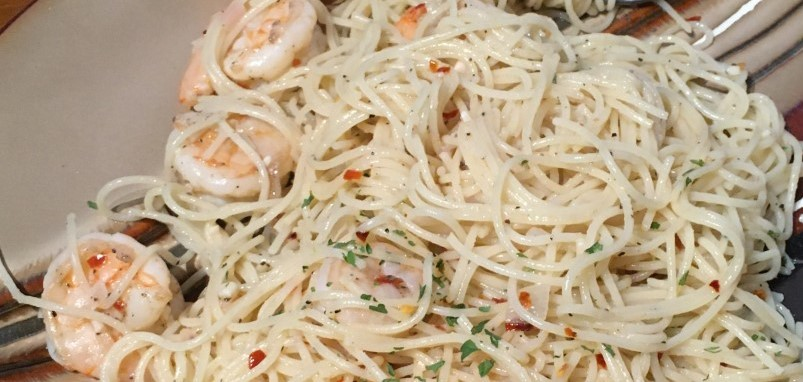
\includegraphics[scale=0.65]{Pasta/Shrimp Scampi/Shrimp Scampi.jpg}
%\end{center}


\end{document}